\section{Verdeckung durch Pointcloud Projektion} \label{sec:pc-projection}

Die erste und weniger aufwändige Idee eine Überlagerung in Augmented Reality zu realisieren, ist die Überführung der Pointcloud in eine Depthmap, die wiederum in den Rendering Prozess mit eingebracht wird. Das Verfahren von \citet{kanbara2000stereoscopic} verfolgt einen ähnlichen Weg mit einer Stereokamera und einer video see-through Displaytechnologie in Form eines Head-Mounted Display. Wie in Abbildung \ref{fig:stereo-depth-map} zu erkennen, bestimmen sie mit Hilfe der Stereokamera Tiefeninformationen, die das gerenderte virtuelle Objekt an den Positionen ausspart, an denen Tiefeninformationen im Vordergrund vorliegen. \\

\begin{figure}[h]
  \centering
	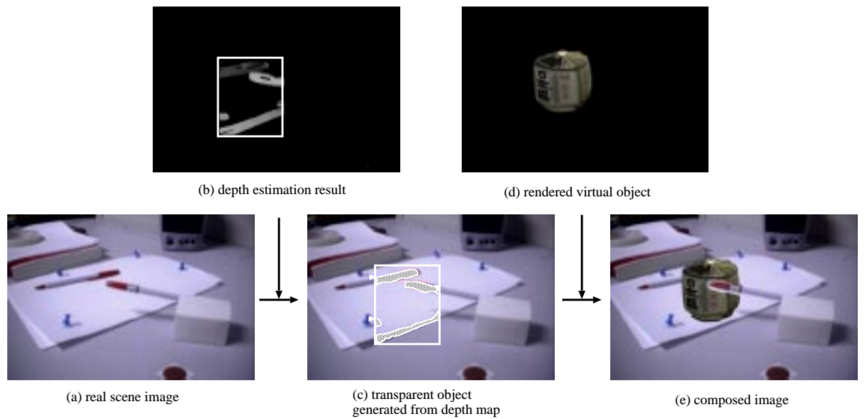
\includegraphics[width=1.0\textwidth]{content/images/methods/stereo-depth-map.png} 
  \caption{Visualisierung des Methode zur Vedeckung durch Depth Maps. Übernommen von \citet{kanbara2000stereoscopic}}
  \label{fig:stereo-depth-map}
\end{figure}

Anders als im oberen Verfahren wird eine Depthmap anhand der vorhandenen Pointcloud aus dem Infrarot Sensor von Project Tango generiert. Dadurch, dass die intrinsischen Kameraeigenschaften der Farbkamera zur Verfügung stehen, welche die Selben der Infrarotkamera sind, können wir einen Punkt \(P = [X, Y, Z]\) der Pointcloud mit der Gleichung \ref{eq:projection} auf die Bildebene überführen. Hier stehen die Variablen \(f_{x/y}\) für Brennweite und \(c_{x/y}\) für den Bildmittelpunkt auf der Bildebene. \citep{Tango90:online}

\begin{equation}\label{eq:projection}
x = X / Z * f_x + c_x
\qquad
y = Y / Z * f_y + c_y
\end{equation}

An dieser Stelle der Depthmap wird nun eine Punkt mit einem Graustufenwert, entsprechend der Entfernung \(|\overrightarrow{PO_{cam}}|\) vom Punkt \(P\) zum Kameraursprung \(O_{cam}\) gezeichnet. Der Farbwert richtet sich dabei nach der Konvention des Rendering Frameworks und den Informationen über die vordere und hintere Clippingebene.\\

Die Auflösung des Tiefensensors der rroject Tango Hardware ist mit \(320x180\) zu \(1280x720\) vier mal kleiner als die Auflösung der Farbkamera ist. Zusätzlich die Dichte der Pointcloud zum eigentlichen Sensor geringer als Ihre eigene Auflösung. So würde man bei einer Auflösung von \(320x180 = 57600\) Tiefenpunkte erwarten. Project Tango liefert jedoch unter guten Bedingungen durchschnittlich \(1700\) Tiefenpunkte. Aufgrund der kleineren Auflösung und der geringeren Informationsdichte werden die gezeichneten Punkte auf der Depthmap hier mit einem Radius von 4 Bildpunkten gezeichnet. \\

Nachdem die Depthmap generiert wurde, kann zum Ausschluss der Pixel der virtuellen Objekte, welches sich hinter einem reellen Objekt befinden, der Z-Buffer Algorithmus aus Kapitel \ref{sec:z-buffer} angewendet werden. Hierzu wird vor dem virtuellen Rendering der Z-Buffer mit den generierten Informationen aus der Depthmap gefüllt. Pixel der virtuellen Objekte werden somit nicht gerendet, wenn nähere Tiefeninformationen realer Objekte and dieser Position vorliegen. 


